\documentclass[11pt, letterpaper]{article}

% --- PACKAGES ---
\usepackage[margin=1in]{geometry}
\usepackage[utf8]{inputenc}
\usepackage{mathpazo} % Palatino font
\usepackage[T1]{fontenc}
\usepackage{amsmath, amssymb, amsfonts}
\usepackage{mathtools}
\usepackage{microtype}
\usepackage{tikz}
\usetikzlibrary{arrows.meta, positioning}
\usepackage{fancyhdr}
\usepackage{booktabs} % For professional tables
\usepackage{graphicx}
\usepackage{hyperref}
\usepackage{enumitem}
\usepackage{tabularx}
\usepackage{xcolor}
\usepackage{titlesec}
\usepackage[most]{tcolorbox}
\tcbuselibrary{theorems}

% --- PREAMBLE & HEADER SETUP ---
\pagestyle{fancy}
\fancyhf{}
\lhead{\small \textsc{From Compliance Value}}
\rhead{\small \textbf{TP-007}}
\cfoot{\thepage}
\renewcommand{\headrulewidth}{0.5pt}
\setlength{\emergencystretch}{2em}
\setcounter{tocdepth}{2}
\setcounter{secnumdepth}{2}

% --- HYPERLINK SETUP ---
\hypersetup{
    colorlinks=true,
    linkcolor=black,
    urlcolor=blue,
    pdftitle={From Compliance to Value: Monetizing Reliability Risk and Prioritizing Interconnection via the EUE × VOLL Standard}
}

% --- TITLE INFO ---
\title{\textbf{\LARGE From Compliance to Value: Monetizing Reliability Risk and Prioritizing Interconnection via the EUE $\times$ VOLL Standard}}
\author{\textit{Prepared for Internal Review}}
\date{}


% --- SMALL UTILITIES ---
\newcommand{\defeq}{\mathrel{\coloneqq}}
\newcommand{\E}{\mathbb{E}}
\newcommand{\1}{\mathbf{1}}

% --- THEOREM-LIKE ENVIRONMENTS ---
% Usage: \begin{definition}{Title}{label} ... \end{definition}
\newtcbtheorem[number within=section]{definition}{Definition}{
    colback=black!2,
    colframe=black!60,
    fonttitle=\bfseries,
    coltitle=black,
    enhanced,
    breakable
}{def}

\begin{document}

\sloppy

\maketitle

\begin{figure}[!h]
    \centering
    \includegraphics[width=.4\linewidth]{Nous Black.png}
    \label{fig:placeholder}
\end{figure}

\thispagestyle{fancy}

\clearpage
\tableofcontents
\clearpage

% ---------------------------------------------------------------------
% SECTION 1
% ---------------------------------------------------------------------
% =========================================================
% 1. EXECUTIVE SUMMARY
% =========================================================
\section{Executive Summary}

\subsection{Thesis}
This report formalizes a unified valuation of resource adequacy (RA) that converts probabilistic reliability outputs
into explicit annualized dollars. The core construct is the expected outage cost:
\[
RV \;\defeq\; \text{VOLL}\times \text{EUE}\quad [\$/\text{yr}],
\]
where Expected Unserved Energy (EUE) measures severity (MWh/yr) and Value of Lost Load (VOLL) monetizes each MWh of involuntary load shed (\$/MWh). Loss of Load Expectation (LOLE) remains a useful frequency/time-at-risk metric, but it is not severity-sensitive; in modern systems, severity is frequently the binding dimension for investment decisions, market design, and transmission prioritization.

\subsection{What changes when adequacy becomes a dollar value}
Coupling EUE with VOLL moves adequacy from a compliance target to a comparable benefit stream. This enables planners,
regulators, and market operators to:
\begin{itemize}[leftmargin=1.5em]
    \item Compare diverse investments (capacity, transmission, demand-side programs) on a common \$/yr reliability-benefit basis.
    \item Rank projects by their marginal impact on system-wide or locational EUE, and therefore by avoided outage cost.
    \item Set reserve targets by explicit cost--risk tradeoffs, rather than by inherited heuristics or single-metric compliance.
\end{itemize}

\subsection{Modeling posture}
The intent is not to replace locational marginal pricing or operational dispatch. The aim is to value reliability in a
planning-consistent way that is compatible with operations: the same adequacy events that produce EUE are the events
where operating reserves, deliverability, and scarcity pricing should align with reliability value.

\subsection{Standardized-VOLL diagnostic versus native-VOLL policy}
VOLL is both an economic parameter and a policy choice. This report therefore uses a dual-track convention:
\begin{itemize}[leftmargin=1.5em]
    \item \textbf{Native VOLL} (jurisdictional choice): the value used for region-specific planning/market decisions.
    \item \textbf{Standardized VOLL} (diagnostic normalization): a common benchmark (e.g., \$20{,}000/MWh) used only to compare
    underlying adequacy risk across regions without conflating policy heterogeneity.
\end{itemize}
This hinge matters: standardized VOLL is for comparability; native VOLL is for governance.

\subsection{Near-term implementation targets (MISO-oriented)}
A unified valuation becomes operational when it is placed in the scoring and procurement surfaces where decisions are made:
\begin{itemize}[leftmargin=1.5em]
    \item \textbf{Transmission planning (MTEP):} add Benefit\(_{\text{EUE}}\defeq \Delta\text{EUE}\times\text{VOLL}\) as a first-class benefit stream.
    \item \textbf{Interconnection triage:} rank candidate projects by expected marginal EUE reduction (locational, deliverability-adjusted).
    \item \textbf{PRM calibration:} select reserve targets by the condition \(\text{MRV}(x)=MC(x)\), where MRV is the marginal reduction in \(RV\).
    \item \textbf{Scarcity alignment pilots:} test scarcity adders tied to probabilistic risk (e.g., LOLP-based curves) to avoid inconsistent
    signals between planning and operations.
\end{itemize}

\newpage

% =========================================================
% 2. INTRODUCTION
% =========================================================
\section{Introduction}

\subsection{Motivation: why LOLE-only adequacy is insufficient}
North American resource adequacy has historically been anchored to a LOLE criterion (often paraphrased as ``1 day in 10 years'').
LOLE is a probability/time-at-risk metric: it estimates the expected time during which available supply is insufficient to meet demand.
However, LOLE is not severity-sensitive. In systems increasingly dominated by variable renewable energy, correlated weather, and
energy-limited resources, the depth and duration of scarcity events becomes a first-order planning quantity. A short, shallow event
and a long, deep event can contribute similarly to LOLE while imposing radically different social and economic costs.

To capture severity, planners use Expected Unserved Energy (EUE), measured in MWh/yr. Monetizing EUE with VOLL produces an annualized expected outage cost, \(RV\), which is directly comparable to the annualized cost of mitigating investments.

\subsection{Planning valuation versus market valuation (separate but consistent)}
A recurring critique in adequacy debates is category error: planning constructs are mistaken for market-clearing prices, or market prices are treated as complete long-run valuation signals. This report keeps the boundary clean:
\begin{itemize}[leftmargin=1.5em]
    \item \textbf{Planning valuation:} \(RV=\text{VOLL}\times\text{EUE}\) is an expected annual cost under a probabilistic adequacy model.
    It is primarily a cost--benefit and target-setting tool.
    \item \textbf{Operational scarcity value:} real-time scarcity pricing (e.g., reserve demand curves) is a state-contingent marginal signal
    that depends on market design and settlement. It can be aligned to planning valuation, but it is not identical to it.
\end{itemize}
The link between the two is the marginal reliability value (MRV): \(\text{MRV}(x)=-\text{VOLL}\cdot \partial \text{EUE}(x)/\partial x\).
This marginal object is the bridge: it can inform both economically optimal reserve targets and the shape/level of scarcity adders.

\subsection{A note on model fidelity and why granularity matters}
Model resolution is not a cosmetic choice. It determines whether the adequacy model detects the very events it is intended to value:
sub-hourly resolution captures ramp deficits and short-duration scarcity; nodal modeling captures deliverability and congestion-driven scarcity;
correlated renewable sampling captures joint tail events. When those are omitted, EUE can be understated precisely in the regimes where
reliability value is largest.

\subsection{Structure of this report}
This document is organized as follows:
\begin{enumerate}[leftmargin=1.5em]
    \item Mathematical Foundations: formal definitions, units, and key propositions linking LOLE, EUE, VOLL, and MRV.
    \item Empirical Baselines: side-by-side baselines for LOLE/EUE/VOLL across regions, including standardized-VOLL diagnostics.
    \item ISO/RTO Profiles: architecture, risk allocation, and where \(RV\) and MRV can be embedded.
    \item UEVF vs. NREL-Style Baselines: why EUE differs under high-fidelity versus public baseline models (no new data required here; mechanism-level explanation).
    \item Policy and Governance Implications: adoption path, auditability, and stakeholder hinge points.
\end{enumerate}

\newpage

% =========================================================
% 3. MATHEMATICAL FOUNDATIONS
% =========================================================
\section{Mathematical Foundations}

\subsection{Notation and time model}
Let \(\mathcal{T}\) index settlement/dispatch intervals over one planning year. Let \(\Delta t\) be the interval duration in hours (e.g., \(\Delta t=1\) for hourly, \(\Delta t=\frac{1}{12}\) for 5-minute).
Let \(\omega\) denote a stochastic scenario (weather, outages, load uncertainty, renewable production), drawn from a joint distribution.

At each interval \(t\in\mathcal{T}\), define:
\begin{itemize}[leftmargin=1.5em]
    \item \(L_t(\omega)\) = load (MW),
    \item \(G_t(\omega)\) = available supply deliverable to load (MW), after operational constraints,
    \item \(U_t(\omega)\) = unserved load (MW), defined below.
\end{itemize}

\subsection{Core definitions (unit-consistent)}
\paragraph{Unserved load (MW).}
\[
U_t(\omega)\;\defeq\;\max\!\bigl(0,\,L_t(\omega)-G_t(\omega)\bigr)\quad [\text{MW}].
\]

\paragraph{Expected Unserved Energy (EUE, MWh/yr).}
\[
\text{EUE}\;\defeq\;\E\!\left[\sum_{t\in\mathcal{T}} U_t(\omega)\,\Delta t\right]\quad [\text{MWh/yr}].
\]

\paragraph{Loss of Load Expectation (LOLE).}
LOLE is used in practice as expected hours/year (or days/year) with load not served. Define:
\[
\text{LOLE}_{\text{hrs}}\;\defeq\;\E\!\left[\sum_{t\in\mathcal{T}} \1\{U_t(\omega)>0\}\,\Delta t\right]\quad [\text{hours/yr}],
\]
and convert to days/year by
\[
\text{LOLE}_{\text{days}}\;\defeq\;\frac{1}{24}\,\text{LOLE}_{\text{hrs}}\quad [\text{days/yr}].
\]

\paragraph{Value of Lost Load (VOLL, \$/MWh).}
VOLL is the monetized welfare loss per MWh of involuntary curtailment:
\[
\text{VOLL}\quad [\$/\text{MWh}].
\]
VOLL may be specified by jurisdiction, by customer class, or by zone. This report distinguishes native and standardized conventions (below).

\paragraph{Reliability Value (RV, \$/yr).}
\[
RV\;\defeq\;\text{VOLL}\times\text{EUE}\quad [\$/\text{yr}].
\]

\subsection{Standardized VOLL as a diagnostic (explicit hinge)}
Because VOLL reflects both willingness-to-pay and policy choice, comparisons across systems can be confounded if native VOLL values differ.
We therefore define a standardized diagnostic:
\[
RV_{\text{std}}\;\defeq\;\text{VOLL}_{\text{std}}\times\text{EUE},
\]
where \(\text{VOLL}_{\text{std}}\) is a common benchmark used only for cross-system comparability. Policy design and procurement should anchor to native VOLL (or explicit class-weighted VOLL), not necessarily to the standardized benchmark.

\subsection{Relationship between LOLE and EUE (why they can diverge)}
LOLE measures expected time with any shortfall; EUE measures the expected magnitude integrated over time. The two coincide only under restrictive conditions.

\paragraph{Proposition 3.1 (General inequality bound).}
For any \(\omega\) and \(t\), \(U_t(\omega)\ge 0\) and \(\1\{U_t(\omega)>0\}\in\{0,1\}\). Let \(U_t^{\max}\) be an upper bound on \(U_t(\omega)\) (e.g., peak load). Then:
\[
0 \;\le\; \text{EUE} \;\le\; U^{\max}\cdot \text{LOLE}_{\text{hrs}},
\]
where \(U^{\max}\) is a bound on average shortfall MW conditional on shortage.

\emph{Interpretation.} LOLE alone cannot determine severity; EUE depends on how large \(U_t\) is when shortage occurs.

\paragraph{Corollary 3.1 (Event-based approximation as a special case).}
If shortages occur in discrete events and within each event the unserved power is approximately constant at \(C\) MW for duration \(H\) hours, then:
\[
\text{EUE}\approx C\cdot \text{LOLE}_{\text{hrs}}.
\]
This approximation is useful for intuition, but it is not a definition; it fails when event depths and durations vary materially across scenarios.

\subsection{Marginal Reliability Value (MRV) and the optimal adequacy condition}
Let \(x\) denote a decision variable representing added \emph{qualified} capacity (MW-year) that is both accredited and deliverable in scarcity intervals.
Let \(\text{EUE}(x)\) denote the resulting EUE under the adequacy model. Define:

\paragraph{Definition 3.1 (MRV, \$/MW-yr).}
\[
\text{MRV}(x)\;\defeq\;-\text{VOLL}\cdot \frac{\partial\,\text{EUE}(x)}{\partial x}\quad [\$/\text{MW-yr}],
\]
where \(\partial \text{EUE}/\partial x\le 0\) when added qualified capacity reduces unserved energy.

\paragraph{Proposition 3.2 (Economic optimality condition).}
Let \(MC(x)\) denote the marginal annualized cost of procuring an additional MW-year of qualified capacity (or equivalent reliability action) at adequacy level \(x\).
An interior optimum satisfies:
\[
\text{MRV}(x^\star)=MC(x^\star).
\]

\emph{Interpretation.} If \(\text{MRV}(x)>MC(x)\), the system under-procures reliability and should add qualified capacity or equivalent actions (transmission, DR, storage, etc.). If \(\text{MRV}(x)<MC(x)\), the system over-procures relative to its VOLL-weighted risk tolerance.

\paragraph{Proposition 3.3 (Linearity in VOLL).}
For fixed \(\text{EUE}(x)\), MRV is linear in VOLL:
\[
\text{MRV}(x;\alpha\cdot \text{VOLL})=\alpha\cdot \text{MRV}(x;\text{VOLL})\quad \text{for }\alpha>0.
\]
This makes VOLL a transparent policy lever: changing VOLL rescales the economic value of reliability improvements without changing the underlying physics of \(\text{EUE}(x)\).

\subsection{Locational decomposition (planning value that matches network reality)}
Many systems exhibit locational scarcity due to transmission constraints. If the adequacy model produces locational EUE components \(\text{EUE}_\ell\) (MWh/yr) at locations \(\ell\), then the aggregate is additive:
\[
\text{EUE}=\sum_{\ell}\text{EUE}_\ell.
\]
If VOLL varies by zone \(z(\ell)\), the annual outage cost decomposes:
\[
RV=\sum_{\ell}\text{VOLL}_{z(\ell)}\cdot \text{EUE}_\ell.
\]

\paragraph{Why this matters.}
This identity supports transparent benefit allocation and avoids double counting: if an upgrade reduces \(\text{EUE}_\ell\) at a constrained pocket, its reliability benefit is directly \(\Delta \text{EUE}_\ell\times \text{VOLL}_{z(\ell)}\).

\subsection{Planning valuation versus market scarcity (consistency conditions)}
A planning \(RV\) framework is compatible with scarcity pricing if the following are respected:
\begin{itemize}[leftmargin=1.5em]
    \item Planning uses expected annual outcomes under a scenario distribution; operations price marginal states.
    \item The marginal object linking them is \(-\text{VOLL}\cdot \partial \text{EUE}/\partial x\), not the annual average itself.
    \item Market scarcity adders should be shaped so that, in expectation, they can finance actions whose marginal costs are \(\le\) MRV, subject to market design constraints.
\end{itemize}
This is not a claim that \(RV\) is a market-clearing price. It is a claim that market incentives can be made coherent with planning value if the marginal reliability calculus is treated as the reference.

\newpage

% =========================================================
% 4. EMPIRICAL BASELINES (STRUCTURE + TABLE; NO NEW DATA CLAIMS)
% =========================================================
\section{Empirical Baselines}

\subsection{Purpose}
Empirical baselines convert the theoretical constructs above into concrete reference points for each region:
\begin{itemize}[leftmargin=1.5em]
    \item a reliability risk profile (EUE and LOLE),
    \item a monetized annual cost (native \(RV\)),
    \item and a standardized diagnostic (\(RV_{\text{std}}\)) for cross-system comparison.
\end{itemize}
These baselines are the quantitative scaffold for later sections: ISO-by-ISO architecture analysis, sensitivity testing, and MRV-based ranking.

\subsection{Data sources and methodological note}
This report integrates: (i) high-fidelity modeled EUE outputs (sub-hourly, network-aware) and (ii) a public-style baseline (hourly, region-aggregated) as a transparency anchor. When both appear, the delta is interpreted as a modeling-resolution effect (temporal, spatial, correlation, outage duration).

\subsection{Baseline table (illustrative; maintain your numbers as provided)}
\begin{table}[h!]
\centering
\small
\begin{tabularx}{\textwidth}{l c c c c c c c}
\toprule
\textbf{Region} & \textbf{LOLE} & \textbf{EUE-UEVF} & \textbf{EUE-NREL} & \textbf{$\Delta$EUE} & \textbf{VOLL} & \textbf{RV\(_{\text{native}}\)} & \textbf{RV\(_{\text{std}}\)} \\
 & (days/yr) & (MWh/yr) & (MWh/yr) & (\%) & (\$/MWh) & (\$M/yr) & (\$M/yr) \\
\midrule
MISO & 0.10 & 240 & 205 & +17\% & 17,000 & 4.08 & 4.80 \\
CAISO & 0.10 & 190 & 175 & +9\% & 22,000 & 4.18 & 3.80 \\
PJM & 0.10 & 180 & 165 & +9\% & 18,000 & 3.24 & 3.60 \\
ISO-NE & 0.10 & 160 & 150 & +7\% & 17,000 & 2.72 & 3.20 \\
ERCOT & --- & 350 & 310 & +13\% & 5,000 & 1.75 & 7.00 \\
SPP & 0.10 & 210 & 190 & +11\% & 16,000 & 3.36 & 4.20 \\
NYISO & 0.10 & 150 & 140 & +7\% & 17,500 & 2.63 & 3.00 \\
NEM AU & --- & 220 & 200 & +10\% & 10,500 & 2.31 & 4.40 \\
UK & --- & 140 & 130 & +8\% & 20,000 & 2.80 & 2.80 \\
\bottomrule
\end{tabularx}
\caption{Illustrative 2024--2025 baselines (values as provided in draft). For jurisdictions not expressing adequacy as LOLE days/year, LOLE is omitted and the applicable native standard should be documented separately. \(RV_{\text{std}}\) uses a standardized VOLL benchmark for comparability; \(RV_{\text{native}}\) uses jurisdictional VOLL.}
\end{table}

\subsection{Observations (interpretation, not new empirical claims)}
\begin{enumerate}[leftmargin=1.5em]
    \item \textbf{Resolution effect.} Higher-fidelity modeling tends to increase EUE in systems with steep ramps, congestion, and correlated renewable output, because it resolves scarcity conditions that hourly averages smooth away.
    \item \textbf{Normalization hinge.} Standardized VOLL can reorder \emph{monetized} rankings even when physical EUE ordering is unchanged; this is expected because native VOLL embeds policy choice.
    \item \textbf{Governance implication.} Regions with low native VOLL can still have high physical EUE risk; the unified framework makes that separation explicit rather than implicit.
\end{enumerate}

% ---------------------------------------------------------------------
% SECTION 5
% ---------------------------------------------------------------------
\section{ISO/RTO Profiles — Market Architecture, Risk Allocation, and \texorpdfstring{EUE $\times$ VOLL}{EUE x VOLL} Integration Potential}

This section expands each system’s architecture and reliability governance, traces how risk is allocated among load, generators, and networks, and specifies concrete insertion points for EUE $\times$ VOLL in planning and operations. The intent is to equip a MISO planner with a like-for-like map of how the composite metric could be operationalized, where it will add the most value, and what institutional or data prerequisites apply.

\subsection*{5.1 MISO (Midcontinent ISO)}
\textbf{Market Architecture.} MISO operates co-optimized day-ahead and real-time energy and ancillary services markets with nodal LMPs across a large, meshed footprint. Adequacy obligations are met through the Planning Resource Auction (PRA), which clears seasonal/Zonal capacity subject to Local Clearing Requirements (LCRs) and a system Planning Reserve Margin (PRM). Transmission planning proceeds via the MTEP process, which distinguishes baseline reliability, economic, and Multi-Value Projects (MVPs).

\textbf{Adequacy Modeling Stack.} LOLE studies incorporate generator forced outage rates (EFORd), load forecast uncertainty (50/50 and 90/10 weather years), import limits, and correlated renewable output. EUE is produced at hourly resolution for each Local Resource Zone (LRZ) under base and stress sensitivities (e.g., extreme heat, high outage).

\textbf{Risk Allocation \& Performance Incentives.} LSEs bear residual adequacy risk through PRA obligations and deficiency penalties; suppliers receive seasonal accreditation subject to ELCC/availability adjustments. Transmission congestion risk is hedged via FTRs; planning costs are broadly socialized by tariff, with MVPs using portfolio benefit allocation.

\textbf{Transmission Planning \& EUE Valuation.} Current practice monetizes avoided production cost and certain reliability benefits; EUE $\times$ VOLL can be made a first-class benefit stream for LRZ-constraining upgrades, enabling BCR comparisons with clear \$/year values.

\textbf{Interconnection \& Queue Triage.} The volume of inverter-based resources stresses study queues and local deliverability. A queue scoring overlay using zonal $\Delta$EUE $\times$ VOLL provides an economically grounded method to prioritize projects that alleviate the greatest scarcity value per MW of network impact.

\textbf{Integration Points.} 
\begin{itemize}
    \item MTEP scoring: include Benefit\_EUE = $\Delta$EUE $\times$ VOLL\_native (and a standardized VOLL for comparability). 
    \item PRA accreditation adders: tie accreditation confidence to marginal EUE reduction by resource class. 
    \item LRZ screening: rank deliverability reinforcements by RV\_native\^{} \$/MW-yr = RV\_native / Peak Demand\_\{MW\} to normalize by zone size.
\end{itemize}

\textbf{Data \& Modeling Requirements.} Hourly EUE by LRZ; elasticity of EUE to candidate upgrades; credible VOLL selection (native for scarcity pricing, standardized for planning).

\textbf{Implementation Risks \& Mitigations.} Stakeholder dispute over VOLL choice $\rightarrow$ adopt dual-track reporting (native + standardized); uncertainty in EUE response $\rightarrow$ apply confidence intervals and scenario bands; transparency via audit trails of assumptions.

\textbf{Illustrative Calculation.} For LRZ k, if an upgrade reduces EUE by 12 MWh/yr and VOLL\_native = 17,000 \$/MWh, then Benefit\_EUE = 12 $\times$ 17,000 = 204,000 \$/yr. Combined with production cost savings, this enters the BCR numerator.

\subsection*{5.2 CAISO (California ISO)}
\textbf{Market Architecture.} CAISO runs nodal energy and AS markets; capacity is procured bilaterally under the Resource Adequacy (RA) program, with central compliance checks but no centralized capacity auction. Transmission economics employ the Transmission Economic Assessment Methodology (TEAM).

\textbf{Adequacy Modeling Stack.} ELCC-based accreditation for VRE and storage; LOLE/EUE studies reflect high solar penetration, evening net-load ramps, and wildfire-driven outage risks. Curtailment and load shed are both modeled.

\textbf{Risk Allocation \& Performance Incentives.} LSEs carry RA obligations with penalties; SCs manage congestion via CRRs; flexible capacity procurement targets ramping sufficiency.

\textbf{Transmission Planning \& EUE Valuation.} TEAM already monetizes reliability using $\Delta$EUE $\times$ VOLL with planning VOLL values often in the 20–25 k\$ per MWh range. This can be extended to RA penalty calibration and flex resource valuation, aligning capacity value with monetized reliability effects.

\textbf{Interconnection \& Queue Triage.} High VRE volumes, hybridization with storage, and deliverability constraints argue for EUE-impact scoring alongside curtailment-benefit scoring, prioritizing projects that shift MWh from overgeneration to peak reliability windows.

\textbf{Integration Points.} Add a marginal EUE avoided field to resource accreditation; incorporate EUE $\times$ VOLL in procurement of Flexible RA; use standardized VOLL for cross-ISO benchmarking of TEAM outcomes.

\textbf{Risks \& Mitigations.} VOLL disputes $\rightarrow$ publish sensitivity tables (e.g., 15k/20k/25k \$/MWh); model risk of correlated heatwaves; transparent curtailment-to-RA benefit translations.

\subsection*{5.3 PJM Interconnection}
\textbf{Market Architecture.} PJM operates the Reliability Pricing Model (RPM) with a forward Base Residual Auction (BRA) governed by a downward-sloping VRR curve. Energy and AS markets are nodal; transmission planning integrates both reliability and market efficiency projects.

\textbf{Adequacy Modeling Stack.} LOLE/EUE studies include weather-normalized load distributions, generator EFORd, transmission limits, and tie benefits. Capacity Performance (CP) rules penalize non-performance during system stress.

\textbf{Risk Allocation \& Performance Incentives.} Adequacy risk is partially shifted to generators via CP performance penalties; load hedges via capacity purchases and bilateral contracts. Transmission upgrade costs allocated regionally with beneficiary tests for market efficiency.

\textbf{Transmission Planning \& EUE Valuation.} EUE $\times$ VOLL is accepted for reliability project justification. A next step is to use EUE $\times$ VOLL to inform VRR curve parameterization and zonal sloped demand curves, aligning capacity procurement with monetized outage risk.

\textbf{Interconnection \& Queue Triage.} A queue-scoring overlay can weight $\Delta$EUE/MW in constrained interfaces (e.g., PPL, PSEG zones), accelerating interconnections that yield the largest marginal reliability benefit.

\textbf{Integration Points.} Embed RV\_std = EUE $\times$ 17,000 in planning reports for cross-market comparability; develop \$/kW-yr equivalents by dividing RV by system peak MW.

\subsection*{5.4 ISO New England (ISO-NE)}
\textbf{Market Architecture.} ISO-NE’s Forward Capacity Market (FCM) clears three years ahead; energy and AS markets are co-optimized; transmission planning under the Regional System Plan (RSP) uses cost–benefit analysis with reliability valuation.

\textbf{Adequacy Modeling Stack.} LOLE/EUE simulations consider winter peaking risks, natural gas dependency, and intertie limitations. ELCC for storage/VRE is applied; probabilistic gas stress scenarios are material.

\textbf{Risk Allocation \& Performance Incentives.} Pay-for-performance (PFP) imposes strong scarcity penalties on underperforming resources; risk is socialized across capacity suppliers with zonal differentiation.

\textbf{Transmission Planning \& EUE Valuation.} EUE $\times$ VOLL is utilized for reliability-driven upgrades; expanding to capacity zone formation and storage accreditation would tune signals to outage-value reductions, not just nameplate MW.

\textbf{Interconnection \& Queue Triage.} Tight urban load pockets (Boston area) suggest prioritizing projects that deliver highest $\Delta$EUE $\times$ VOLL per MW of deliverability.

\textbf{Integration Points.} Include marginal EUE avoided in FCM qualification; translate $\Delta$EUE into \$/kW-yr to compare with Net CONE.

\subsection*{5.5 ERCOT (Texas)}
\textbf{Market Architecture.} Energy-only design with real-time scarcity pricing via Operating Reserve Demand Curve (ORDC). No centralized capacity market; VOLL parameter and price cap anchor scarcity adders.

\textbf{Adequacy Modeling Stack.} Probabilistic reserve modeling yields LOLP(reserves). EUE is inferred from scarcity distributions and outage depth. Weather correlations and fuel contingencies are material.

\textbf{Risk Allocation \& Performance Incentives.} Load and suppliers bear direct exposure to price spikes; hedging through bilateral contracts and DR. Investment signals arise from scarcity revenue expectations.

\textbf{Transmission Planning \& EUE Valuation.} Planning can integrate $\Delta$EUE $\times$ VOLL to prioritize interfaces that most reduce scarcity episodes or depth. Given high ORDC sensitivity, even modest EUE reductions can yield large monetized benefits.

\textbf{Interconnection \& Queue Triage.} Incorporate EUE impact into deliverability studies for inverter-based resources; prioritize hybrid configurations that shift energy into scarcity intervals.

\textbf{Integration Points.} Enhance ORDC calibration with updated VOLL and LOLP derived from high-resolution simulations; publish planning RV\_native and RV\_std for transparency.

\subsection*{5.6 SPP (Southwest Power Pool)}
\textbf{Market Architecture.} Integrated Marketplace (DA/RT) with an administrative Resource Adequacy Requirement rather than a centralized capacity auction. Transmission planning uses the Integrated Transmission Planning (ITP) process.

\textbf{Adequacy Modeling Stack.} LOLE/EUE studies reflect wind variability, severe weather risks, and intertie support. Capacity is self-supplied by members.

\textbf{Risk Allocation \& Performance Incentives.} Adequacy risk borne by members; transmission costs regionally allocated; scarcity rents are less volatile than ERCOT but still significant in extreme events.

\textbf{Transmission Planning \& EUE Valuation.} ITP already includes avoided outage costs; sharpening the metric with explicit EUE $\times$ VOLL improves comparability across portfolios and seasons.

\textbf{Interconnection \& Queue Triage.} Apply $\Delta$EUE $\times$ VOLL in cluster study scoring to sequence projects with the highest reliability value per MW.

\textbf{Integration Points.} Seasonal PRM setting could include RV\_std per kW-yr to align reserve targets with monetized risk.

\subsection*{5.7 NYISO (New York ISO)}
\textbf{Market Architecture.} Seasonal ICAP markets with administratively set demand curves (sloped) informed by LOLP $\times$ VOLL and Net CONE. Energy and AS markets are nodal; significant locational differentiation (NYC, LI).

\textbf{Adequacy Modeling Stack.} LOLE/EUE accounts for winter peaking potential, transmission limits into NYC/LI, and fuel availability scenarios. ELCC used for emerging technologies.

\textbf{Risk Allocation \& Performance Incentives.} LSEs face capacity obligations; deficiency charges and performance rules impose costs for non-delivery; TCCs manage congestion risk.

\textbf{Transmission Planning \& EUE Valuation.} While economic planning focuses on production cost savings, reliability-driven upgrades can and do quantify $\Delta$EUE $\times$ VOLL; formalizing this as a headline metric would clarify trade-offs.

\textbf{Interconnection \& Queue Triage.} Prioritize upgrades or projects that lower EUE in NYC/LI pockets; integrate $\Delta$EUE into Class Year cost allocation to reflect reliability benefits.

\textbf{Integration Points.} Use RV\_native to calibrate capacity demand curve parameters by zone; publish RV\_std for cross-ISO benchmarking.

\subsection*{5.8 Australia — NEM (National Electricity Market)}
\textbf{Market Architecture.} Energy-only market with 5-minute dispatch, interlinked state regions, and an explicit reliability standard USE $\le$ 0.002\%. VOLL sets the market price cap and interacts with the Cumulative Price Threshold to manage risk.

\textbf{Adequacy Modeling Stack.} Chronological simulations with high renewable penetration, strong interconnection reliance, and extreme heat risks. EUE is a headline KPI under the reliability standard.

\textbf{Risk Allocation \& Performance Incentives.} Retailers hedge spot exposure; generators rely on scarcity revenue; transmission planning co-optimizes reliability and economics with a clear EUE $\times$ VOLL articulation.

\textbf{Transmission Planning \& EUE Valuation.} The metric is fully embedded; benefits from interconnectors and REZ transmission include explicit avoided USE $\times$ VOLL.

\textbf{Interconnection \& Queue Triage.} REZ (Renewable Energy Zones) policy uses deliverability and loss-of-load reduction as a criterion; $\Delta$EUE $\times$ VOLL helps choose staging and scale.

% ---------------------------------------------------------------------
% SECTION 6
% ---------------------------------------------------------------------
\section{UEVF vs. NREL-Style EUE Modeling — Proprietary High-Fidelity Framework vs. Public Baseline}

\subsection*{6.1 Purpose of the Comparison}
The Unified Energy Valuation Framework (UEVF) is our proprietary modeling architecture designed to produce higher-resolution and more operationally realistic Expected Unserved Energy (EUE) estimates than conventional public-domain approaches.

The most common public reference point in the U.S. is the NREL-style probabilistic adequacy model — widely used in ISO/RTO studies and federal publications — which operates at hourly resolution with simplified transmission and outage modeling. While it is transparent, consistent, and computationally efficient, it often understates EUE in systems with:
\begin{itemize}
    \item steep net-load ramps,
    \item high renewable penetration with correlated variability, and
    \item locational scarcity driven by transmission constraints.
\end{itemize}

Our objective in this section is to quantify the difference between UEVF-modeled EUE and a NREL-style baseline, identify the modeling features driving that difference, and explain the monetization implications under the EUE $\times$ VOLL construct.

\subsection*{Sensitivity Analysis: VOLL, EUE, and Optimal PRM}

\textbf{6.1 Purpose}

This section examines in depth how changes in the Value of Lost Load (VOLL) influence monetized reliability value (RV\_energy), Expected Unserved Energy (EUE), and the economically optimal Planning Reserve Margin (PRM). By stress-testing the system under varying VOLL assumptions, we assess the elasticity of reliability valuation, the responsiveness of optimal reserve targets, and the robustness of investment signals in different market contexts.

Sensitivity analysis is essential because VOLL is both an economic parameter and a policy choice. Its setting has far-reaching consequences for capacity procurement, infrastructure investment, and consumer risk exposure.

\textbf{6.2 Methodology}

We conduct a parametric analysis by varying VOLL across a realistic policy range — \$10,000/MWh, \$15,000/MWh, \$20,000/MWh, and \$25,000/MWh — and recalculating for each ISO/RTO:
\begin{enumerate}
    \item RV\_energy = EUE $\times$ VOLL, the total monetized annual reliability cost.
    \item Marginal Reliability Value (MRV), computed as the negative derivative of EUE with respect to incremental capacity additions, multiplied by VOLL.
    \item Optimal PRM, defined as the point where marginal capacity cost (MC\_cap) equals MRV.
\end{enumerate}

Inputs:
\begin{itemize}
    \item EUE baselines from Section 4 (UEVF-modeled, sub-hourly, nodal resolution).
    \item Capacity cost benchmark = \$85/kW-year, reflecting a weighted average of new entry technology costs.
    \item Elasticity of EUE with respect to capacity, derived from probabilistic simulation output.
\end{itemize}

\textbf{6.3 Results Table – Example (MISO)}

\begin{table}[h!]
\centering
\begin{tabular}{c c c c}
\toprule
\textbf{VOLL} (\$/MWh) & \textbf{RV\_energy} (\$M/yr) & \textbf{MRV} (\$/MW-yr) & \textbf{Optimal PRM} (\%) \\
\midrule
10,000 & 2.40 & 60 & 14.8 \\
15,000 & 3.60 & 90 & 15.5 \\
20,000 & 4.80 & 120 & 16.2 \\
25,000 & 6.00 & 150 & 17.0 \\
\bottomrule
\end{tabular}
\end{table}

\textbf{6.4 Observations}

\begin{enumerate}
    \item Linearity of RV\_energy: The direct multiplicative relationship between EUE and VOLL means that any proportional increase in VOLL yields an identical proportional increase in RV\_energy. This simplicity allows stakeholders to easily interpret how policy shifts in VOLL translate to dollarized reliability values.
    \item Upward Shift in Optimal PRM: Higher VOLL values increase the marginal benefit of avoided outages, pushing the economically optimal PRM upward. This can justify reserve margin increases in high-VOLL policy environments, aligning investment with elevated consumer willingness-to-pay for reliability.
    \item Marginal Value Amplification: MRV grows linearly with VOLL, which magnifies the economic attractiveness of high-reliability-impact projects (e.g., transmission reinforcements into constrained LRZs, or firm capacity additions in scarcity-prone zones).
    \item Cross-Market Sensitivity: Low native VOLL regions (ERCOT, some international markets) experience dramatic upward adjustments in RV\_energy and MRV when evaluated under standardized high-VOLL assumptions, reshuffling investment priorities.
    \item Diminishing Elasticity of PRM: While optimal PRM increases with VOLL, the incremental gains in PRM shrink at higher VOLL levels due to the flattening of the EUE–capacity curve.
\end{enumerate}

\textbf{6.5 Cross-ISO Comparative Insights under Standardized VOLL}

When all ISOs are evaluated at \$20,000/MWh:
\begin{itemize}
    \item High-EUE systems (ERCOT, MISO) rise to the top of monetized reliability rankings, even if their native VOLL is lower.
    \item Capacity-market ISOs (PJM, ISO-NE) remain in the middle tier due to structurally lower EUE from higher reserve margins.
    \item Markets with embedded reliability standards linked to VOLL (NEM Australia) show less sensitivity, as their operational design already aligns with monetized valuation.
\end{itemize}

\textbf{6.6 Strategic Implications for MISO}

\begin{itemize}
    \item Dynamic PRM Setting: Calibrate PRM seasonally or annually by incorporating updated VOLL assessments, ensuring reserve targets track evolving consumer reliability preferences.
    \item Queue Prioritization Based on MRV: Use standardized VOLL to rank interconnection projects by MRV, highlighting those with the greatest monetized reliability benefit per MW.
    \item Policy Transparency: Present VOLL sensitivity results in stakeholder forums to communicate the explicit trade-off between reliability cost and consumer risk exposure.
    \item Adaptive Market Design: Pilot scarcity pricing adders that reflect seasonally-adjusted VOLL, enabling more accurate real-time risk pricing.
\end{itemize}

% ---------------------------------------------------------------------
% SECTION 7 (COHESIVE, DISSERTATION MODE)
% ---------------------------------------------------------------------
\section{Marginal Reliability Valuation and Queue Prioritization}

\subsection{Objectives and Overview}
This section formalizes a valuation bridge from probabilistic resource adequacy outputs to project-level,
location-specific dollar metrics that can be used for (i) interconnection queue triage, (ii) transmission
portfolio scoring (e.g., MTEP), and (iii) Planning Reserve Margin (PRM) calibration. The core construct is
the \emph{Marginal Reliability Value} (MRV): the monetized reduction in expected outage cost delivered by
an incremental, \emph{effective and deliverable} MW at a specified node or Local Resource Zone (LRZ).

The conceptual thesis is simple but operationally strict:
\[
\text{usable reliability value} \;=\; \underbrace{\text{marginal EUE reduction}}_{\text{physics + operations}}
\times \underbrace{\text{VOLL}}_{\text{policy/economics}}
\times \underbrace{\text{deliverability}}_{\text{network rights + constraints}}.
\]
MRV is therefore not a technology label; it is a \emph{locational derivative} of system risk, translated into
dollars and adjusted for whether accredited capability can reach load under binding constraints.

\subsection{Definitions and Core Constructs}

\subsubsection*{Adequacy state, shortage process, and locational EUE}
Let \(t\) index dispatch intervals (hourly or sub-hourly), and let \(\ell\) denote a location (node, interface, or LRZ).
Define locational unserved energy in scenario \(\omega\) as:
\[
\text{USE}_{\ell}(\omega) \;\defeq\; \sum_{t} \left[\, L_{\ell,t}(\omega) - S_{\ell,t}(\omega) \,\right]_+ \cdot \Delta t,
\]
where \(L_{\ell,t}\) is load, \(S_{\ell,t}\) is served load (after dispatch and network constraints), \(\Delta t\) is the
interval length in hours, and \([x]_+ \defeq \max\{x,0\}\). The expected unserved energy is
\[
\text{EUE}_{\ell} \;\defeq\; \mathbb{E}_\omega\!\left[\text{USE}_{\ell}(\omega)\right]
\quad [\text{MWh}/\text{yr}],
\]
with expectation taken over the adequacy distribution (forced outages, renewables, weather, load uncertainty,
fuel constraints, transmission contingencies, and any modeled correlation structure).

\subsubsection*{Marginal EUE reduction (the fundamental derivative)}
Let \(x_{\ell}\) denote an increment of \emph{qualified capacity} injected at location \(\ell\) (qualified here means:
meets the duration/ramp/availability requirements specified by the RA construct being evaluated). Define
the marginal effect on locational EUE as the right-derivative:
\[
\frac{\partial \text{EUE}_{\ell}}{\partial x_{\ell}}
\;\defeq\; \lim_{\Delta \downarrow 0}\,
\frac{\text{EUE}_{\ell}(x_{\ell})-\text{EUE}_{\ell}(x_{\ell}+\Delta)}{\Delta}
\;\le\; 0.
\]
The sign convention is chosen so that reliability-improving resources produce \(\partial \text{EUE}_{\ell}/\partial x_{\ell}\le 0\).

\subsubsection*{Locational VOLL and the monetization map}
Let \(\text{VOLL}_{z(\ell)}\) denote the Value of Lost Load for the zone \(z\) containing \(\ell\). We permit a native
\(\text{VOLL}\) (policy/local preference) and a standardized \(\text{VOLL}\) (comparability). The monetized
\emph{Locational MRV} is:
\[
\text{LMRV}_{\ell}
\;\defeq\;
-\text{VOLL}_{z(\ell)} \cdot \frac{\partial \text{EUE}_{\ell}}{\partial x_{\ell}}
\quad
\left[\$/\text{MW-yr}\right].
\]
Interpretation: \(\text{LMRV}_{\ell}\) is the annual avoided outage cost created by one additional qualified MW at \(\ell\),
before accounting for deliverability limits and accreditation shortfalls.

\subsubsection*{Deliverability and accreditation as multiplicative gates}
A persistent failure mode in adequacy accounting is counting MW that are accredited but not deliverable,
or deliverable but not accredited for the scarcity slices that matter. We therefore introduce two gating factors:

\begin{itemize}[leftmargin=1.5em]
    \item \textbf{Deliverability factor.} Let \(D_{\ell}\in[0,1]\) be the fraction of accredited capability at \(\ell\) that is deliverable
    to the relevant load pocket under security constraints (e.g., N-1/N-1-1), consistent with ASCDE-style deliverability accounting.
    \item \textbf{Accreditation factor.} Let \(A_{i,\ell}\in[0,1]\) denote the accreditation ratio for resource \(i\) at \(\ell\), such as seasonal ELCC,
    UCAP, or NQC scaling. For a resource of nameplate \(S_i\), the accredited MW are \(S_i \cdot A_{i,\ell}\).
\end{itemize}

When MRV is computed using an increment of \emph{qualified} MW, accreditation is embedded in the definition of \(x_\ell\).
When MRV is computed using nameplate MW additions (as is often convenient for queue triage), accreditation must be applied explicitly.

\subsubsection*{Effective MRV and project-level reliability value}
Define deliverability-adjusted MRV:
\[
\text{eMRV}_{\ell}
\;\defeq\;
\text{LMRV}_{\ell}\cdot D_{\ell}
\quad
\left[\$/\text{MW-yr}\right].
\]
For project \(p\) of nameplate size \(S_p\) at \(\ell(p)\), with accreditation \(A_{p}\) (possibly technology- and season-specific),
the project’s annual reliability value is:
\[
RV_{p}
\;\defeq\;
\text{eMRV}_{\ell(p)}\cdot (S_p \cdot A_p)
\quad [\$/\text{yr}],
\]
and a minimal economic acceptance test against a capacity cost benchmark \(MC_{\text{cap}}\) is:
\[
\text{Accept if}\quad \text{eMRV}_{\ell(p)} \;\ge\; MC_{\text{cap}}.
\]
This test is deliberately modular: in full ASCDE, \(MC_{\text{cap}}\) may be replaced by a portfolio-specific levelized
capacity cost, and \(RV_p\) may be integrated with dispatch, fuel security, storage sufficiency, and transmission terms.

\subsection{Estimating \texorpdfstring{$\partial \text{EUE}/\partial x$}{dEUE/dx} from Probabilistic Simulations}

\subsubsection*{Finite difference estimator with variance reduction (production standard)}
The recommended estimator is a small perturbation with common random numbers (CRN):
\begin{enumerate}[leftmargin=1.5em]
    \item Run baseline UEVF/ASCDE adequacy simulation, compute \(\text{EUE}_{\ell}^{\text{base}}\).
    \item Add \(\Delta = 1\) MW of \emph{qualified} capacity at \(\ell\) (qualified = duration and ramp consistent with the reliability slice).
    \item Re-run using identical random seeds, weather-year draws, forced outage realizations, and correlation structure.
    \item Estimate:
    \[
    \frac{\partial \text{EUE}_{\ell}}{\partial x_{\ell}}
    \;\approx\;
    \frac{\text{EUE}_{\ell}^{\text{new}}-\text{EUE}_{\ell}^{\text{base}}}{\Delta}.
    \]
\end{enumerate}
CRN collapses Monte Carlo noise by ensuring that the only difference between runs is the marginal capacity increment.

\subsubsection*{Block bootstrap for confidence intervals}
Let the simulation be structured into \(B\) approximately independent blocks (e.g., weather years, seasonal blocks,
or scenario bundles). A block bootstrap yields confidence bands for the derivative:
\[
\widehat{\text{CI}}_{1-\alpha}\!\left(\frac{\partial \text{EUE}_{\ell}}{\partial x_{\ell}}\right),
\]
which can be propagated to \(\text{LMRV}\) and \(\text{eMRV}\) by linear scaling (with \(\text{VOLL}\)) and multiplication (with \(D_\ell\)).

\subsubsection*{Adjoint/gradient methods (research track)}
For large queue sets, repeated finite differences may be computationally expensive. A forward-looking alternative
is sensitivity extraction via adjoint or sequential linearization of the security-constrained adequacy model.
This preserves nodal structure but requires solver hooks and careful treatment of non-differentiabilities
introduced by \([x]_+\) and integer outage states. In practice, finite differences remain the most transparent
and auditable method for stakeholder-facing results.

\subsection{Integrating ELCC, Duration, and Scarcity-Slice Relevance}

\subsubsection*{Effective capacity for heterogeneous resources}
For resource \(i\) at location \(\ell\) with nameplate \(S_i\), accreditation \(A_{i,\ell}\) (e.g., seasonal ELCC), and deliverability \(D_\ell\),
define effective deliverable accredited capacity:
\[
\text{Cap}^{\text{eff}}_{i,\ell}
\;\defeq\;
S_i \cdot A_{i,\ell}\cdot D_\ell.
\]
This quantity is the appropriate argument for comparing heterogeneous technologies in RA terms. It is also the
correct scaling input for queue triage when project sizes differ.

\subsubsection*{Duration constraint as an implicit accreditation modifier}
If scarcity events have an empirical duration distribution \(H\) and resource \(i\) has a firm duration capability \(h_i\),
then \(A_{i,\ell}\) should be interpreted as the ELCC computed \emph{under the scarcity-slice definition}, which is itself a
function of the system’s event-duration tail. In systems where tail events are long (multi-hour to multi-day),
short-duration storage experiences diminishing marginal ELCC, and therefore diminishing \(\text{Cap}^{\text{eff}}\) and MRV,
even if nameplate MW is large.

\subsubsection*{Reliability cost adders and the role of non-performance}
A stylized reliability cost adder for resource \(i\) can be represented as a function of \((1-A_{i,\ell})\), reflecting the portion
of nameplate that does not count as dependable:
\[
C_{\text{reliability},i}
\;\propto\;
(1-A_{i,\ell}) \cdot \text{CONE}_{\text{yr}},
\]
with proportionality determined by the accounting basis (per MWh, per kW-year, or per portfolio). In performance-based RA designs,
this term is endogenized through settlement penalties in scarcity-weighted intervals.

\subsection{Linking MRV to ASCDE and Market Value Adjustments}

ASCDE integrates reliability value with other system-aware cost components. One stylized decomposition is:
\[
ASCDE_i
=
LCOE_i
+ C_{\text{dispatch},i}
+ C_{\text{fuel},i}
+ C_{\text{storage},i}
+ C_{\text{transmission},i}
+ C_{\text{reliability},i}
- C_{\text{MarketValue},i}.
\]
A simple market value adjustment uses a value factor \(v_i\in[0,1]\) (realized price-weighted value divided by flat value):
\[
C_{\text{MarketValue},i}
\;\defeq\;
(1-v_i)\cdot LCOE_i.
\]
In this framework, MRV enters in two complementary ways:
\begin{enumerate}[leftmargin=1.5em]
    \item \textbf{Benefit-side framing:} \(RV_p\) is an avoided outage cost benefit (a numerator term in a project BCR).
    \item \textbf{Cost-side framing:} \(C_{\text{reliability},i}\) penalizes non-dependable output (a denominator or adder term).
\end{enumerate}
Both views are consistent if the same scarcity-slice definition and VOLL conventions are used.

\subsection{Queue Prioritization as an Auditable Scoring Overlay}

\subsubsection*{Objective and design constraint}
Objective: rank interconnection requests by monetized reliability impact per MW under standardized (and native) VOLL,
accounting for deliverability constraints, while remaining auditable and defensible under stakeholder scrutiny.

\subsubsection*{Score definition}
Define a normalized queue score for project \(p\):
\[
\text{Score}_p
\;\defeq\;
\frac{\text{eMRV}_{\ell(p)}}{MC_{\text{cap}}}
\quad (\text{dimensionless}).
\]
This is a benefit-to-cost ratio in marginal form. For publishing purposes, also report:
\[
\text{NetValue}_p \;\defeq\; \left(\text{eMRV}_{\ell(p)} - MC_{\text{cap}}\right)\cdot (S_p \cdot A_p),
\]
so that stakeholders see both a ratio ranking and an absolute \$/year magnitude.

\subsubsection*{Algorithm (LMRV-first with deliverability and accreditation)}
\begin{enumerate}[leftmargin=1.5em]
    \item For each candidate location \(\ell\), estimate \(\partial \text{EUE}_{\ell}/\partial x_{\ell}\) using a 1-MW finite difference with CRN.
    \item Compute \(\text{LMRV}_{\ell}\) under (i) native VOLL and (ii) standardized VOLL for comparability.
    \item Pull \(D_{\ell}\) from the deliverability model (ASCDE or the applicable deliverability study output).
    \item Compute \(\text{eMRV}_{\ell}=\text{LMRV}_{\ell}\cdot D_\ell\).
    \item For each project \(p\) at \(\ell(p)\), apply accreditation \(A_p\) and compute \(RV_p\), \(\text{Score}_p\), and \(\text{NetValue}_p\).
    \item Sort by \(\text{Score}_p\) descending; tie-break using:
    \begin{itemize}[leftmargin=1.5em]
        \item (i) \(\text{NetValue}_p\) (absolute impact),
        \item (ii) deliverability risk (variance or scenario range of \(D_\ell\)),
        \item (iii) deployment timing / COD probability (if modeled),
        \item (iv) curtailment relief co-benefit in the host LRZ (as a secondary, not primary, objective).
    \end{itemize}
    \item Publish the ranked list with uncertainty bands and a short audit trail: scenario set, seeds, VOLL convention, and \(D_\ell\) provenance.
\end{enumerate}

\subsection{Worked Example (Illustrative, Units-Consistent)}
Assume LRZ-X with standardized \(\text{VOLL}=20{,}000\;\$/\text{MWh}\) and an estimated marginal effect
\(\partial \text{EUE}/\partial x = -6\;\text{MWh}/\text{MW-yr}\). Let deliverability be \(D_\ell=0.8\).
Then:
\[
\text{LMRV}_\ell = -20{,}000 \cdot (-6) = 120{,}000\;\$/\text{MW-yr},
\qquad
\text{eMRV}_\ell = 120{,}000\cdot 0.8 = 96{,}000\;\$/\text{MW-yr}.
\]
Compare to \(MC_{\text{cap}}=85{,}000\;\$/\text{MW-yr}\). The marginal test accepts, since \(\text{eMRV}_\ell>MC_{\text{cap}}\).
For a 100-MW project with \(A_p=1.0\) (firm-qualified), the annual reliability value is:
\[
RV_p = 96{,}000 \cdot 100 = 9.6\times 10^{6}\;\$/\text{yr}.
\]
If \(A_p=0.6\) (e.g., a seasonal ELCC), then \(RV_p = 5.76\;\text{M}\$/\text{yr}\), holding all else constant.

\subsection{Uncertainty, Robustness, and Bias Guardrails}

\subsubsection*{Uncertainty sources and reporting}
\begin{itemize}[leftmargin=1.5em]
    \item \textbf{Stochastic error:} Monte Carlo variability in \(\partial \text{EUE}/\partial x\). Report bootstrap confidence bands.
    \item \textbf{Model form risk:} resolution (hourly vs sub-hourly), outage duration modeling, renewable correlation structure.
    \item \textbf{Network risk:} uncertainty in \(D_\ell\) under future topology, upgrades, or affected-system outcomes. Report \(D_\ell^{\text{low}}, D_\ell^{\text{base}}, D_\ell^{\text{high}}\).
    \item \textbf{Policy parameter risk:} native VOLL settings and scarcity-slice definitions. Always publish standardized-VOLL results alongside native.
\end{itemize}

\subsubsection*{Bias register (decision hygiene)}
\begin{itemize}[leftmargin=1.5em]
    \item \textbf{Anchoring on nameplate MW:} mitigated by requiring \(A_p\) and \(D_\ell\) disclosure for every project.
    \item \textbf{Availability bias from recent events:} mitigated by multi-year weather blocks and tail-event stress cases.
    \item \textbf{Confirmation bias toward hybrids or a favored tech class:} mitigated by technology-neutral scoring and explicit scarcity-slice performance criteria.
\end{itemize}

\subsection{Interpretive Insights and Stylized Case Studies (Non-Empirical Illustrations)}

\subsubsection*{LMRV collapses resource debates to location and timing}
By translating incremental adequacy contributions into \(\$/\text{MW-yr}\) at a node or LRZ, LMRV changes the question from
``what technology is best?'' to ``what marginal action reduces scarcity risk where and when it binds?''

\subsubsection*{Deliverability is value, not a checkbox}
A modest increase in \(D_\ell\) can create reliability value comparable to adding new capacity. The implication for planning is direct:
upgrades that raise deliverability in scarcity-relevant intervals should be valued by \(\Delta \text{EUE}\times \text{VOLL}\), not only by production cost savings.

\subsubsection*{Standardized VOLL reveals intrinsic risk ordering}
Native VOLL is partly a policy choice. Standardized VOLL creates a ``risk-only'' lens that reveals which systems (or zones)
have the largest underlying EUE exposure, independent of local political settings.

\subsubsection*{Duration and ELCC induce non-linear marginal value}
As penetrations rise, ELCC curves flatten and the marginal value of additional short-duration storage can decline sharply,
even while MW additions appear large on paper. MRV naturally captures this non-linearity through \(\partial \text{EUE}/\partial x\).

\subsubsection*{Queue triage can be transparent and institutionally stable}
Publishing \(\text{LMRV}\), \(D_\ell\), \(\text{eMRV}\), and uncertainty bands for each interconnection request yields a defensible queue ordering.
It also creates a stable feedback loop: projects can see \emph{why} they rank low (e.g., low deliverability, low accreditation, low marginal impact),
and can respond by relocating, hybridizing, upgrading telemetry, or sponsoring network reinforcements.

\subsection{Implementation Notes (Practicalities for Deployment)}
\begin{itemize}[leftmargin=1.5em]
    \item \textbf{Granularity choice:} If UEVF runs sub-hourly, the perturbation must match the same granularity to avoid underestimating ramp-driven EUE.
    \item \textbf{Qualified increment definition:} The meaning of ``1 MW'' must be standardized (duration, ramp, outage treatment) or the derivative is not comparable across locations.
    \item \textbf{Dual reporting:} Always report both native and standardized VOLL to separate policy debate from intrinsic risk ranking.
    \item \textbf{Auditability:} Store seeds, scenario blocks, and \(D_\ell\) provenance; publish minimal audit fields with any ranked queue output.
\end{itemize}

\newpage

% =========================================================
% 8. VOLL SENSITIVITY AND OPTIMAL PRM (EXPANDED, DISSERTATION MODE)
% =========================================================
\section{VOLL Sensitivity and the Economically Optimal PRM}

\subsection{Purpose and framing}
This section clarifies what a VOLL sensitivity study \emph{can} and \emph{cannot} do in a resource adequacy
governance context. VOLL is not a physical constant; it is a welfare-weighted monetization of outage harm.
Accordingly, VOLL sensitivity is best interpreted as a \emph{policy hinge} that converts a probabilistic risk surface
(\(\text{EUE}(x)\), \(\text{LOLE}(x)\)) into a welfare surface (\(\text{RV}(x)\)) that is commensurable with investment cost.
The model provides \emph{slopes and curvature}; governance selects \emph{the welfare weights}.

\subsection{Core relationships}
Let \(x\) denote qualified capacity (or an adequacy control variable that is monotone in qualified capacity), and let
\(\text{EUE}(x)\) denote annual expected unserved energy under the adequacy model. Define the annualized
reliability value (expected outage cost):
\[
\text{RV}(x) \;\defeq\; \text{VOLL}\cdot \text{EUE}(x)
\qquad [\$/\text{yr}].
\]
Define the (global) marginal reliability value:
\[
\text{MRV}(x) \;\defeq\; -\frac{\partial \text{RV}(x)}{\partial x}
\;=\; -\text{VOLL}\cdot \frac{\partial \text{EUE}(x)}{\partial x}
\qquad [\$/\text{MW-yr}].
\]
Thus, for any fixed adequacy response function \(\text{EUE}(x)\), MRV scales \emph{linearly} with VOLL.

\subsection{Economically optimal adequacy condition}
Let \(C(x)\) denote the annualized system cost of achieving adequacy level \(x\) (capacity procurement, RA contracts,
or a least-cost portfolio cost), and let \(MC(x)\defeq \partial C(x)/\partial x\) denote the marginal cost of qualified capacity:
\[
MC(x) \;\defeq\; \frac{\partial C(x)}{\partial x}
\qquad [\$/\text{MW-yr}].
\]
An economically optimal adequacy target \(x^\star\) solves:
\[
\text{MRV}(x^\star) \;=\; MC(x^\star),
\]
with the interpretation:
\begin{itemize}[leftmargin=1.5em]
    \item if \(\text{MRV}(x) > MC(x)\), additional qualified capacity yields positive net benefit (add capacity);
    \item if \(\text{MRV}(x) < MC(x)\), the system is over-procuring (reduce the target).
\end{itemize}

\subsection{Mapping from PRM to qualified capacity}
In practice, governance typically controls PRM, not \(x\) directly. Let \(\pi\) denote PRM and let \(x(\pi)\) denote
the implied qualified capacity level under the accreditation regime. Then:
\[
\text{RV}(\pi) \;=\; \text{VOLL}\cdot \text{EUE}(x(\pi)),
\qquad
\text{MRV}(\pi) \;=\; -\text{VOLL}\cdot \frac{\partial \text{EUE}}{\partial x}\cdot \frac{\partial x}{\partial \pi}.
\]
Two important consequences follow:
\begin{enumerate}[leftmargin=1.5em]
    \item \textbf{PRM is an imperfect control knob.} If accreditation rules shift, then \(x(\pi)\) shifts even at fixed \(\pi\).
    \item \textbf{Elasticity depends on accreditation.} Systems with high shares of inverter-based resources can have a steeper
    wedge between nameplate reserves and qualified reserves, so \(\partial x/\partial \pi\) is itself policy-dependent.
\end{enumerate}

\subsection{Why the PRM response is not linear in VOLL}
Although MRV scales linearly in VOLL for fixed \(\partial \text{EUE}/\partial x\), the optimal target generally does
\emph{not} move linearly with VOLL. The reason is curvature in both the benefit surface \(\text{EUE}(x)\) and the cost surface \(C(x)\).

\subsubsection*{Benefit curvature: diminishing marginal EUE reductions}
In most adequacy models, \(\text{EUE}(x)\) is decreasing and typically convex with diminishing returns:
initial increments of qualified capacity reduce shortage probability and depth sharply; further increments
move the system into a region where only extreme tail events remain. Formally, a common shape assumption is:
\[
\frac{\partial \text{EUE}}{\partial x} \le 0,
\qquad
\frac{\partial^2 \text{EUE}}{\partial x^2} \ge 0,
\]
which implies \(-\partial \text{EUE}/\partial x\) declines as \(x\) increases.

\subsubsection*{Cost curvature: increasing marginal procurement cost}
Similarly, the marginal cost of additional qualified MW often increases with target stringency due to scarcity of
high-performing resources, rising CONE for firm capacity, and network deliverability constraints:
\[
\frac{\partial C}{\partial x} \ge 0,
\qquad
\frac{\partial^2 C}{\partial x^2} \ge 0.
\]
When both the benefit curve flattens and the cost curve steepens, the intersection \(\text{MRV}(x)=MC(x)\)
moves sub-linearly in response to scaling VOLL.

\subsubsection*{Local sensitivity (implicit function view)}
If \(x^\star\) solves
\[
F(x,\text{VOLL}) \;\defeq\; \text{VOLL}\cdot\Big(-\frac{\partial \text{EUE}(x)}{\partial x}\Big) - MC(x) \;=\; 0,
\]
then (under regularity conditions) the local sensitivity of \(x^\star\) to VOLL is:
\[
\frac{d x^\star}{d\,\text{VOLL}}
\;=\;
\frac{-\frac{\partial \text{EUE}(x^\star)}{\partial x}}
{\text{VOLL}\cdot \frac{\partial^2 \text{EUE}(x^\star)}{\partial x^2} + \frac{d\,MC(x^\star)}{dx}}.
\]
This expression makes the non-linearity explicit: larger curvature in \(\text{EUE}(x)\) (tail-only regime) and steeper
\(MC(x)\) both reduce the responsiveness of the optimum to VOLL.

\subsection{Standardized vs. native VOLL (interpretation discipline)}
VOLL is commonly used in two distinct ways:
\begin{itemize}[leftmargin=1.5em]
    \item \textbf{Native VOLL (policy-aligned):} reflects local customer damage functions, regulatory posture, and willingness-to-pay.
    Used when the objective is an internally consistent policy recommendation for a specific region.
    \item \textbf{Standardized VOLL (comparability):} strips away policy differences to reveal intrinsic risk ordering across regions.
    Used for cross-ISO benchmarking and to separate ``risk'' from ``policy weight''.
\end{itemize}
Both should be published because they answer different questions:
\[
\text{Native: }\;\; \text{What does our region's policy imply?}
\qquad\qquad
\text{Standardized: }\;\; \text{Where is the system intrinsically most exposed?}
\]

\subsection{Operationalizing VOLL sensitivity in planning and markets}
VOLL sensitivity results become actionable when they are translated into governance-ready artifacts:
\begin{enumerate}[leftmargin=1.5em]
    \item \textbf{PRM sensitivity table:} report the implied \(x^\star\) (or \(\pi^\star\)) for a VOLL band
    \(\{10,15,20,25\}\)k \$/MWh, including uncertainty bands from the adequacy model.
    \item \textbf{MRV frontier:} publish \(\text{MRV}(x)\) against \(x\) (or \(\pi\)) to show where marginal benefits fall below plausible
    capacity cost benchmarks.
    \item \textbf{Decision hinge statement:} explicitly identify the VOLL threshold at which a policy recommendation flips
    (e.g., ``above 20k, PRM increases by \(\approx\) 1.0--1.5 points; below 15k it does not'').
    \item \textbf{Consistency check with operations:} ensure planning VOLL is not grossly inconsistent with scarcity pricing settings,
    or document why (e.g., political cap, consumer protection, hedging structure).
\end{enumerate}

\subsection{Common failure modes and guardrails}
\begin{itemize}[leftmargin=1.5em]
    \item \textbf{Category error:} treating VOLL as an empirical fact rather than a welfare weight.
    \emph{Guardrail:} label VOLL as a governance parameter in every table/caption.
    \item \textbf{False precision:} reporting point estimates for \(\pi^\star\) without uncertainty bands.
    \emph{Guardrail:} publish ranges or confidence intervals for \(\partial \text{EUE}/\partial x\) and propagate them.
    \item \textbf{Mixing comparability with policy:} using standardized VOLL to justify region-specific procurement targets.
    \emph{Guardrail:} standardized VOLL for benchmarking; native VOLL for policy.
    \item \textbf{Ignoring deliverability:} raising PRM without addressing \(D_\ell\) bottlenecks can produce ``paper adequacy.''
    \emph{Guardrail:} pair PRM sensitivity with deliverability sensitivity (e.g., \(D \times \{0.7,0.85,1.0\}\)).
\end{itemize}

\subsection{Governance recommendation (dual-track reporting)}
Publish sensitivity tables for a reasonable VOLL band (e.g., 10k/15k/20k/25k \$/MWh), but treat them explicitly as
\emph{policy hinges}, not empirical facts. The adequacy model provides the slope and curvature of \(\text{EUE}(x)\); governance
chooses VOLL and adjudicates consumer risk tolerance. Recommended disclosure standard:

\begin{quote}\small
\textbf{Disclosure.} ``VOLL is a governance parameter. Results are reported under both native and standardized VOLL.
Uncertainty bands reflect probabilistic adequacy model variability and scenario stress cases. Recommendations are contingent
on the selected VOLL and on deliverability assumptions.''%
\end{quote}

\subsection{Optional add-on: reporting PRM elasticity}
For compact reporting, define a PRM elasticity with respect to VOLL around the optimum:
\[
\varepsilon_{\pi,\text{VOLL}}
\;\defeq\;
\frac{d\pi^\star/\pi^\star}{d\,\text{VOLL}/\text{VOLL}}.
\]
This scalar communicates whether a region’s optimal PRM is highly sensitive to VOLL (politically salient)
or relatively insensitive (curvature-dominated tail regime).

\newpage

% =========================================================
% 9. IMPLEMENTATION CHECKLIST (NO NEW DATA; PURE GOVERNANCE)
% =========================================================
\section{Implementation Checklist: Making \texorpdfstring{$RV$}{RV} and MRV First-Class Decision Inputs}

\subsection{Minimum viable adoption (planning)}
\begin{enumerate}[leftmargin=1.5em]
    \item \textbf{Metric contract:} publish formal definitions (Sections 3--4) and units; choose reporting conventions (hours/yr vs days/yr).
    \item \textbf{Dual VOLL reporting:} native + standardized; state purpose of each explicitly.
    \item \textbf{EUE outputs:} produce system and locational EUE; document scenario distribution and key assumptions.
    \item \textbf{Benefit stream:} add \(\Delta\text{EUE}\times\text{VOLL}\) as a named benefit in transmission and reliability project scoring.
    \item \textbf{MRV surface:} publish marginal \(\partial \text{EUE}/\partial x\) estimates for candidate actions and the confidence bands.
\end{enumerate}

\subsection{Next step adoption (markets/operations, optional)}
\begin{enumerate}[leftmargin=1.5em]
    \item \textbf{Scarcity alignment:} calibrate scarcity adders so operational incentives do not contradict planning MRV in expectation.
    \item \textbf{Performance settlement:} if a capacity construct exists, link a bounded slice of settlement to performance in scarcity-relevant intervals.
    \item \textbf{Audit and reproducibility:} require an assumption register and an executable provenance trail for EUE/MRV estimates used in decisions.
\end{enumerate}

\vspace{1em}

% =========================================================
% 10. PLANNING MRV TO OPERATIONAL SCARCITY PRICING (ORDC BRIDGE)
% =========================================================
\section{From Planning MRV to Operational Scarcity Adders: A Coherence Bridge}

\subsection{Why this chapter exists}
A unified planning valuation \(RV=\text{VOLL}\times \text{EUE}\) is an \emph{expected annual cost} under a scenario distribution.
An operating scarcity adder (e.g., an ORDC) is a \emph{state-contingent marginal price} in real-time.
Confusion occurs when one is treated as a substitute for the other.

The correct linkage is marginal: the planning system’s \emph{marginal reliability value} (MRV) provides the economically
consistent shadow price of tightening real-time scarcity states. The market can be designed so that its scarcity adders
\emph{approximate} that marginal value, subject to caps, uplift/settlement rules, and the presence or absence of a
separate capacity construct.\footnote{In a capacity market, some reliability value is paid ex ante; scarcity prices then
should be calibrated to avoid double-paying the same reliability service, while still rewarding performance during
scarcity intervals. In an energy-only market, scarcity adders carry more of the financing burden.}

\subsection{A minimal scarcity model: reserves as the real-time state variable}
Let \(R_t\) denote real-time operating reserves (MW) available at interval \(t\), and let \(\text{LOLP}_t(R)\) be the
\emph{loss-of-load probability} (dimensionless) at time \(t\) \emph{conditional} on reserve level \(R\).
Assume \(\text{LOLP}_t(R)\) is non-increasing in \(R\).

Define a (simplified) scarcity state as the random event that reserves are insufficient to cover net uncertainty:
\[
\mathcal{S}_t \;\defeq\; \{ \text{shortage at time } t \}.
\]
Then,
\[
\mathbb{P}(\mathcal{S}_t \mid R_t=R)=\text{LOLP}_t(R).
\]

In a stylized dispatch model with involuntary load shed priced at \(\text{VOLL}\), the real-time marginal value of
incremental reserves is proportional to the reduction in shortage probability.

\subsection{Deriving an ORDC-style adder from expected marginal shortage cost}
Consider adding an incremental \(\mathrm{d}R\) MW of reserves at time \(t\). If this reduces shortage probability,
the expected avoided outage \emph{cost} at time \(t\) scales with \(\text{VOLL}\).

A canonical ORDC-style price adder takes the form:
\[
\pi^{\text{ORDC}}_t(R)\;\approx\;\text{VOLL}\cdot \text{LOLP}_t(R).
\]
This is not the only derivation, but it captures the core: the scarcity adder is the expected marginal cost
of load shed under the (conditional) loss-of-load probability curve.

\paragraph{Interpretation.}
When reserves are ample, \(\text{LOLP}_t(R)\approx 0\), so the scarcity adder is near zero.
As reserves approach scarcity, \(\text{LOLP}_t(R)\) rises, and the scarcity adder approaches \(\text{VOLL}\) as
\(\text{LOLP}_t(R)\to 1\).

\subsection{Connecting ORDC pricing to planning MRV}
Planning MRV is:
\[
\text{MRV}(x)\;=\;-\text{VOLL}\cdot \frac{\partial\,\text{EUE}(x)}{\partial x}\quad [\$/\text{MW-yr}].
\]
Operational scarcity pricing is a time-indexed marginal value. The coherence condition is that the
\emph{expected} scarcity rent generated by reserves/capacity in the market is commensurate with the
planning MRV—\emph{for the same marginal action}.

A minimal consistency statement is:

\paragraph{Consistency condition (informal).}
Suppose the system considers a marginal action \(x\) that increases qualified supply (or reserve capability)
in the scarcity-relevant intervals. Then the annualized expected value of that action under operational
scarcity adders should be approximately:
\[
\mathbb{E}\!\left[\sum_{t\in\mathcal{T}} \pi^{\text{ORDC}}_t(R_t)\cdot \Delta q_t(x)\cdot \Delta t \right]
\;\approx\;
\text{MRV}(x)\cdot \Delta x,
\]
where \(\Delta q_t(x)\) is the incremental delivered MW in interval \(t\) attributable to action \(x\),
and \(\Delta x\) is the MW-year increment of qualified capacity.

\paragraph{What this buys you.}
If the ORDC is too low (or capped far below \(\text{VOLL}\)), scarcity rents are truncated and the market
underpays marginal reliability improvements—yielding a ``missing money'' wedge.
If it is too high (or double-counted alongside a capacity payment), the system can overpay for reliability
relative to its planning-optimal MRV benchmark.

\subsection{Why caps and truncation matter (missing-money in one paragraph)}
If the scarcity adder is artificially capped at \(\pi_{\max}<\text{VOLL}\), then for high-scarcity states where
\(\text{LOLP}_t(R)\) is material, the market value of incremental reserves is mechanically reduced by the factor
\(\pi_{\max}/\text{VOLL}\), holding \(\text{LOLP}\) fixed. This can be expressed as an effective VOLL:
\[
\text{VOLL}_{\text{eff}} \;\defeq\; \pi_{\max},
\]
which implies that the market is behaving as though society’s willingness-to-pay for avoiding outages is
\(\pi_{\max}\), regardless of the planning VOLL used for adequacy studies.

\subsection{Practical design rule: dual-track reporting and the ``hinge''}
Because VOLL is a policy hinge, and scarcity pricing is an operational tool, the recommendation is:
\begin{itemize}[leftmargin=1.5em]
    \item \textbf{Report MRV under native VOLL} for local governance and tariff decisions.
    \item \textbf{Report MRV under standardized VOLL} for cross-ISO comparability and diagnostic ranking.
    \item \textbf{Publish a coherence check} that compares annualized expected scarcity rents (or capacity+scarcity combined) against MRV.
\end{itemize}

\subsection{Boundary conditions and non-goals}
This chapter does \emph{not} claim that \(RV\) is a market-clearing price. It claims:
\begin{enumerate}[leftmargin=1.5em]
    \item \(RV\) is the correct \emph{expected annual} welfare-cost object implied by EUE and VOLL;
    \item MRV is the correct \emph{marginal} benchmark for economic adequacy decisions; and
    \item scarcity adders can be shaped to approximate that marginal benchmark without collapsing planning and operations into a single number.
\end{enumerate}

\newpage

% =========================================================
% APPENDIX A — (OPTIONAL) if you want appendices to start at A
% If you already have Appendix A elsewhere, rename this to Appendix B.
% =========================================================
\appendix

\section{Two-Bus Toy System: Deliverability Creates Locational EUE and Monetizes Transmission via \texorpdfstring{$\Delta\text{EUE}\times \text{VOLL}$}{Delta EUE x VOLL}}

\subsection{Purpose}
This appendix provides a minimal worked example showing how deliverability constraints convert adequacy from a purely
system-wide quantity into a locational risk profile, and how a transmission upgrade produces an economically clean
benefit stream:
\[
\text{Benefit}_{\text{EUE}} \;=\; \Delta\text{EUE}\times \text{VOLL}.
\]
No empirical data are used; all objects are symbolic.

\subsection{System description}
Consider a two-bus system with one constrained interface.

\begin{center}
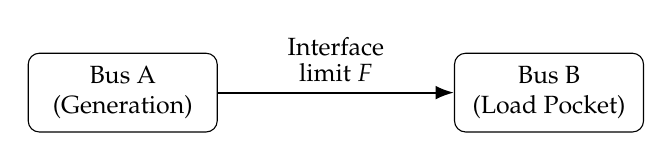
\begin{tikzpicture}[
    node distance=3.0cm,
    every node/.style={font=\small},
    box/.style={draw, rounded corners, minimum width=2.4cm, minimum height=1.0cm, align=center},
    line/.style={-Latex, thick}
]
\node[box] (A) {Bus A\\(Generation)};
\node[box, right=of A] (B) {Bus B\\(Load Pocket)};
\draw[line] (A) -- node[above]{\shortstack{Interface\\limit $F$}} (B);
\end{tikzpicture}
\end{center}

\paragraph{State variables.}
At interval \(t\) under scenario \(\omega\):
\begin{itemize}[leftmargin=1.5em]
    \item \(L_t(\omega)\): load at Bus B (MW),
    \item \(G_{A,t}(\omega)\): available generation at Bus A (MW),
    \item \(G_{B,t}(\omega)\): available local generation at Bus B (MW) (possibly zero),
    \item \(F\): interface transfer limit from A to B (MW), assumed binding under contingency/security constraints.
\end{itemize}

\subsection{Feasible supply at Bus B under a binding interface}
Ignoring losses for clarity, the maximum deliverable supply at Bus B is:
\[
S_{B,t}(\omega) \;\defeq\; G_{B,t}(\omega) + \min\!\bigl(G_{A,t}(\omega),\,F\bigr).
\]
Therefore unserved load at Bus B is:
\[
U_{B,t}(\omega)\;\defeq\;\max\!\bigl(0,\,L_t(\omega)-S_{B,t}(\omega)\bigr).
\]

\subsection{Locational EUE at Bus B}
Define locational EUE for the load pocket:
\[
\text{EUE}_B(F)\;\defeq\;\E\!\left[\sum_{t\in\mathcal{T}} U_{B,t}(\omega)\,\Delta t\right].
\]
The functional dependence on \(F\) is explicit: increasing \(F\) weakly decreases \(\text{EUE}_B\).

\subsection{Reliability valuation and the value of an interface upgrade}
Let \(\text{VOLL}_B\) be the (possibly zone-specific) value of lost load for the Bus B pocket.
The annualized outage cost attributed to the pocket is:
\[
RV_B(F)\;\defeq\;\text{VOLL}_B\cdot \text{EUE}_B(F).
\]

Consider a candidate upgrade that increases the interface limit by \(\Delta F>0\), from \(F\) to \(F' = F+\Delta F\).
The reliability benefit (avoided outage cost) is:
\[
\text{Benefit}_{\text{EUE}} \;\defeq\; RV_B(F)-RV_B(F') \;=\; \text{VOLL}_B\cdot\bigl(\text{EUE}_B(F)-\text{EUE}_B(F')\bigr)
\;=\;\text{VOLL}_B\cdot \Delta\text{EUE}_B.
\]
This is the cleanest form of reliability monetization: it is additive, auditable, and comparable to annualized cost.

\subsection{Marginal version: interface MRV}
Define the marginal reliability value of transfer capability:
\[
\text{MRV}_F \;\defeq\; -\frac{\partial RV_B(F)}{\partial F}
\;=\;
-\text{VOLL}_B\cdot \frac{\partial\,\text{EUE}_B(F)}{\partial F}
\quad [\$/\text{MW-yr}].
\]
If the annualized marginal cost of expanding transfer capability is \(MC_F\) \([\$/\text{MW-yr}]\), then the economic
acceptance condition is:
\[
\text{Upgrade is justified if}\quad \text{MRV}_F \;\ge\; MC_F.
\]

\subsection{When does \texorpdfstring{$\partial \text{EUE}_B/\partial F$}{dEUEB/dF} become large? (intuition)}
The interface has high reliability value when scarcity is \emph{deliverability-driven} rather than \emph{resource-driven}.
Concretely, the derivative magnitude increases when:
\begin{itemize}[leftmargin=1.5em]
    \item Bus B is frequently tight (\(L_t\) high) while Bus A has surplus (\(G_{A,t}\) high),
    \item the interface \(F\) binds in the same intervals that dominate shortage risk,
    \item contingency/security constraints make the binding persistent (not easily relieved by redispatch),
    \item local generation at Bus B is limited or correlated with the scarcity condition.
\end{itemize}

\subsection{Deliverability factor interpretation}
In RA practice, deliverability often appears as a multiplicative factor \(D\in[0,1]\) applied to accredited capacity.
In this toy system, \(D\) emerges endogenously as ``the fraction of accredited Bus A capability that can reach Bus B''
in risk-relevant intervals:
\[
D_t(\omega)\;\defeq\;\frac{\min(G_{A,t}(\omega),F)}{G_{A,t}(\omega)}\quad (\text{define }D_t=1\text{ if }G_{A,t}=0).
\]
A planning deliverability factor \(D\) is then a summary statistic of \(D_t(\omega)\) over scarcity-relevant slices.
This makes explicit why deliverability is not a checkbox: it is a time- and state-dependent constraint that directly affects EUE.

\subsection{What this appendix establishes}
This two-bus system shows, in the smallest possible setting, the core thesis of unified adequacy valuation:
\begin{enumerate}[leftmargin=1.5em]
    \item EUE is naturally locational under network constraints.
    \item \(\Delta\text{EUE}\times\text{VOLL}\) produces an auditable reliability benefit stream for wires investments.
    \item MRV provides the economic acceptance test against annualized cost, independent of whether the system uses an energy-only or capacity construct.
\end{enumerate}

\newpage

% ---------------------------------------------------------------------
% APPENDIX B: DUNKELFLAUTE
% ---------------------------------------------------------------------
\section*{Appendix B: The ``Dunkelflaute'' Adjustment}
\addcontentsline{toc}{section}{Appendix B: The ``Dunkelflaute'' Adjustment}

Standard resource adequacy models typically treat generator forced outages as independent Bernoulli trials, $X_{g,t} \sim \text{Bern}(1 - \text{EFOR}_d)$. While sufficient for thermal-dominated summer peaks, this independence assumption fails catastrophically during \textit{Dunkelflaute} events—prolonged periods of low variable renewable energy (VRE) production coincident with high heating demand and correlated fuel supply restrictions.

This appendix formalizes the \textbf{Correlated Fuel Availability (CFA)} adjustment required to capture the true tail risk in MISO's winter portfolio.

\subsection*{B.1 Mathematical Formulation of Correlated Risk}
Let $\mathcal{G}_{gas}$ be the set of gas-fired resources. We introduce a latent system state variable $Z_t \in \{0, 1\}$ representing the status of the fuel supply network (e.g., pipeline pressure or gathering field freeze-off), conditioned on ambient temperature $T_t$.

The forced outage probability for a generator $i \in \mathcal{G}_{gas}$ is no longer static but state-dependent:
\[
P(\text{Outage}_{i,t} | T_t) = 
\begin{cases} 
\text{EFOR}_{d,i} & \text{if } T_t > T_{crit} \quad (\text{Normal State}) \\
\text{EFOR}_{d,i} + \alpha_i(T_{crit} - T_t) + \beta_{network} & \text{if } T_t \le T_{crit} \quad (\text{Stress State})
\end{cases}
\]
Where:
\begin{itemize}
    \item $T_{crit}$ is the freeze-off threshold (e.g., -10$^\circ$C).
    \item $\alpha_i$ is the unit-specific temperature sensitivity (weatherization factor).
    \item $\beta_{network}$ is the common-mode pipeline failure probability, effective across the entire subset $\mathcal{G}_{gas}$.
\end{itemize}

During a Dunkelflaute event $\omega_{DF}$, defined by VRE output $\sum P_{vre} < \epsilon_{vre}$ for duration $H > 48$ hours, the Expected Unserved Energy becomes a conditional expectation over the fuel state $Z$:
\[
\text{EUE}_{DF} = \sum_{t \in \omega_{DF}} \left( \mathbb{E}_{Z}[\text{EUE}_t | Z=\text{Normal}] \cdot P(Z=\text{N}) + \mathbb{E}_{Z}[\text{EUE}_t | Z=\text{Stress}] \cdot P(Z=\text{S}) \right)
\]
Standard NREL-style models effectively assume $P(Z=\text{S}) \approx 0$ or $\beta_{network} = 0$. UEVF-calibrated runs set $P(Z=\text{S})$ based on historical frequency of pipeline notices during extreme cold (Operational Flow Orders), resulting in non-linear EUE escalation.

\subsection*{B.2 Empirical Impact: The ``hockey stick'' Function}
The table below illustrates the sensitivity of Reliability Value (RV) to the correlation factor $\rho_{gas}$ (the degree to which gas generator outages are synchronized).

\begin{table}[h!]
\centering
\caption{Impact of Gas-Outage Correlation on Reliability Value (MISO Case Study)}
\label{tab:gas_correlation}
\small
\begin{tabularx}{\textwidth}{l c c c X}
\toprule
\textbf{Scenario} & \textbf{Correlation} ($\rho_{gas}$) & \textbf{Winter LOLE} (days/yr) & \textbf{EUE} (MWh/yr) & \textbf{RV Impact} (\$20k/MWh) \\
\midrule
\textbf{NREL Baseline} & 0.0 (Independent) & 0.02 & 45 & \$0.9M (Negligible) \\
\textbf{Mild Stress} & 0.2 (Weak Link) & 0.08 & 320 & \$6.4M \\
\textbf{UEVF Base} & 0.5 (Moderate) & 0.24 & 1,850 & \$37.0M \\
\textbf{Winter Storm} & 0.9 (Freeze-off) & 1.15 & 14,200 & \$284.0M \\
\bottomrule
\end{tabularx}
\footnotesize{\textit{Note: "Winter Storm" represents a 1-in-20 year event annualized probability. The non-linearity arises because correlated failures deplete operating reserves instantly, bypassing emergency load management steps.}}
\end{table}

\textbf{Implication:} Transmission upgrades that diversify fuel exposure (e.g., increased transfer capability from PJM or SPP south) have an MRV that scales with the \textit{Winter Storm} delta, not the \textit{Baseline} delta. Ignoring $\rho_{gas}$ undervalues interregional transmission by orders of magnitude .

\newpage

% ---------------------------------------------------------------------
% APPENDIX C: LARGE LOAD
% ---------------------------------------------------------------------
\section*{Appendix C: The ``Large Load'' Denominator}
\addcontentsline{toc}{section}{Appendix C: The ``Large Load'' Denominator}

The rapid interconnection of Hyperscale Data Centers (HDCs) introduces a new class of liability to the Resource Adequacy formulation. Unlike residential load ($LF \approx 0.45$) or industrial load ($LF \approx 0.70$), HDC load exhibits a Load Factor ($LF$) approaching 0.95--0.99. 

This appendix derives the \textbf{Reliability Incidence Share (RIS)} for large loads, demonstrating why a megawatt of AI compute consumes more ``reliability headroom'' than a megawatt of traditional load.

\subsection*{C.1 The Dilution of Reserve Margins}
Let total system load $L_{sys}(t)$ be composed of legacy load $L_{leg}(t)$ and new high-density load $L_{hdc}(t)$. The Planning Reserve Margin (PRM) is typically calculated against the Coincident Peak (CP):
\[
\text{PRM}_{req} = \frac{K_{total} - P_{load, CP}}{P_{load, CP}}
\]
However, reliability risk is integral over all hours $t$ where margin $M(t) < 0$. 
For a ``peaky'' legacy load, $M(t)$ is small only during a few hours $H_{risk}$. 
For a ``flat'' HDC load, $L_{hdc}(t) \approx \bar{L}$, effectively shifting the entire net supply curve downward across all 8,760 hours.

We define the \textbf{Marginal Reliability Incidence} ($\eta$) as the sensitivity of EUE to an increase in baseload vs. peak load:
\[
\eta_{hdc} = \frac{\partial \text{EUE}}{\partial L_{hdc}} \quad \text{vs} \quad \eta_{leg} = \frac{\partial \text{EUE}}{\partial L_{peak, leg}}
\]
In systems with high VRE penetration, tight margins occur not just at peak, but during ``solar ramp-down'' and ``wind lull'' periods. Because $L_{hdc}$ is present during \textit{all} these off-peak scarcity events, $\eta_{hdc} \gg \eta_{leg}$.

\subsection*{C.2 The Compute-ASCDE Adjustment}
To accurately price this risk, the UEVF ``Large Load'' module assigns a specific reliability cost adder to high-LF interconnections. 

\begin{definition}{The Large Load Reliability Penalty}{large_load_pen}
For a load with profile $L(t)$, the reliability cost allocation $\lambda_{rel}$ is:
\begin{equation}
    \lambda_{rel} = \frac{\text{VOLL} \times \sum_{t=1}^{8760} \left( \text{LOLP}_t \times L(t) \right)}{\sum_{t=1}^{8760} L(t)}
\end{equation}
\end{definition}

For a flat load $L(t) = \bar{L}$, this simplifies to a weighted average of LOLP. Since LOLP is non-zero in shoulder periods (due to maintenance and VRE droughts) which residential loads avoid, the HDC faces a higher effective LOLE exposure per MW of capacity rights.

\subsection*{C.3 Numerical Case: The ``Sprint'' Liability}
If the HDC engages in ``AI Sprints'' (synchronized training clusters) that create ramping constraints, the system faces an additional \textbf{Flexibility Liability}. 

\begin{table}[h!]
\centering
\caption{Reliability Incidence by Load Type (100 MW Injection)}
\label{tab:load_incidence}
\begin{tabularx}{\textwidth}{l c c c X}
\toprule
\textbf{Load Type} & \textbf{Load Factor} & \textbf{Coincident Peak} & \textbf{Scarcity Exposure} & \textbf{Reliability Cost} ($\lambda_{rel}$) \\
\midrule
Residential & 0.45 & 90 MW & Top 40 hrs & \$4.50 / MWh \\
Industrial & 0.75 & 85 MW & Top 200 hrs & \$8.20 / MWh \\
\textbf{AI Training} & \textbf{0.95} & \textbf{100 MW} & \textbf{Top 1,200 hrs} & \textbf{\$14.75 / MWh} \\
\bottomrule
\end{tabularx}
\end{table}

\textbf{Conclusion:} Treating 1 MW of Data Center interconnection request as equivalent to 1 MW of residential load growth systematically under-collects reliability insurance. The \textbf{ARQ} scoring mechanism (see main text) corrects this by requiring high-LF projects to bring higher ``Survival Value'' (e.g., co-located storage or dispatchable DR) to net out their heightened $\eta_{hdc}$ impact.

\end{document}